\documentclass[letterpaper,11pt]{article}

\usepackage[margin=1in]{geometry}
\usepackage[titletoc,title]{appendix}
\usepackage{amsmath}
\usepackage{amssymb}
\usepackage{amsthm}
\usepackage{amscd}
\usepackage{amsfonts}
\usepackage{graphicx}%
\usepackage{fancyhdr}
\usepackage{color}
\usepackage{sectsty}
\usepackage[colorlinks=true,linkcolor=black,anchorcolor=black,citecolor=black,filecolor=black,menucolor=black,runcolor=black,urlcolor=black]{hyperref}
\usepackage{siunitx}
\usepackage{cleveref}
% \usepackage{natbib}
% \usepackage{biblatex} %Imports biblatex package
% \addbibresource{PDR.bib} %Import the bibliography file
\usepackage{csquotes}
\usepackage{array}

%-----------------------------------------------

\hyphenation{LArTPC}
\hyphenation{LArTPCs}

\newcommand{\tslarpaas}      {t_{\text{SLArpaas}}}
\newcommand{\davg}           {d_{\text{avg}}}

%---------------------------------------------

\renewcommand{\arraystretch}{1.2}

%-----------------------------------------------

\pagestyle{fancy}\lhead{}
\setlength{\parindent}{0em}

\title{SLArpaas Engineering Note}
\author{Yun-Tse Tsai}

%-----------------------------------------------

\begin{document}

\maketitle
\tableofcontents

%------------------------------------------------
% Main text
% -----------------------------------------------
\section{Instroduction}
\label{sec:intro}

This engineering note describes a cryogenic vessel's suitability for use in 
a SLAC LDRD project for liquid-argon time-projection chamber (LArTPC) research
and development,
seeking approval for its use at SLAC.\\

The Fundamental Physics Directorate (FPD) DUNE group at SLAC had developed 
and operated two liquid argon cryogenic systems for neutrino detector R\&D
in the Liquid Noble Test Facility (LNTF) at IR2 (building 620).
The Stage One system, LAIR2, consists of a 65-liter cryogenic vessel and
a high voltage test setup,
while the Stage Two system, SLArchetto, includes a 264-liter liquid argon
cryogenic vessel with a time-projection chamber (TPC).\\

The scientists in the DUNE and LZ groups are embarking on Stage Three,
SLArPAAS I (SLAC (LAr) Prototype Ar Assembly System I),
which involves a 60-liter liquid argon cryogenic vessel and a TPC.
The lead physicist is Yun-Tse Tsai, while the lead physicist for the cryogenic
and piping system is Miriam Moore.
The ESH coordinator supporting them is Richard Delacruz.\\

The SLArPAAS I main dewar is a commercially available item manufactured by Cryofab
in New Jersey.
This is a reputable manufacturer with a long history of providing cryogenic vessels 
for scientific research. 
However, the vessels manufactured by Cryofab do not normally come with an ASME stamp. 
This engineering note has been developed to demonstrate its suitability for use in 
this experiment and seek approval for its use at SLAC.\\

The top plate of the vessel was designed by SLAC scientist Brian Lenardo
and was manufactured by Kurt J. Lesker.\\

The supporting documents described in this Note are either directly included in 
the Appendices or accessible online from the links indicated in this Note.\\

\section{System Description}
\label{sec:system}

The Piping and Instrumentation Diagram (P\&ID) of the three stages
of the systems is shown in Fig.~\ref{fig:PID}.

% ----------------------------------------------------------
\begin{figure}[h]
    \centering
    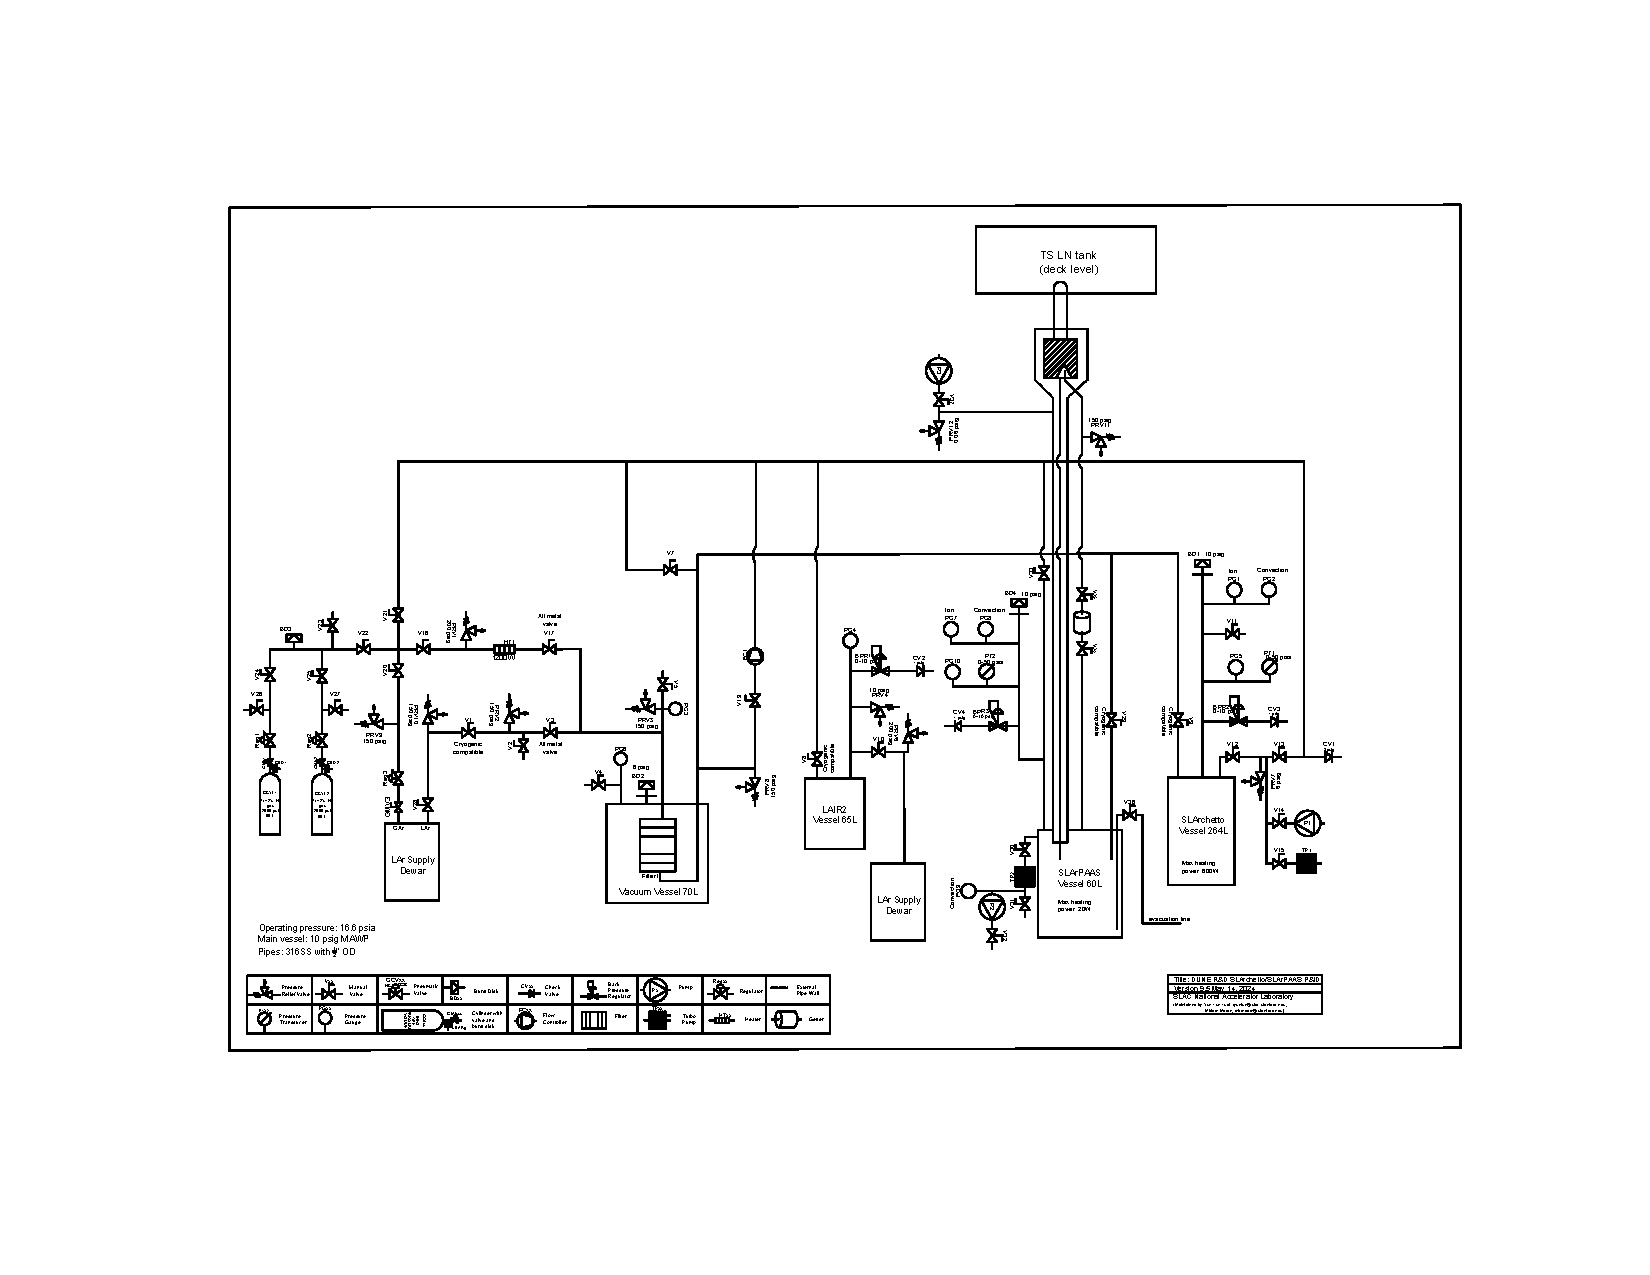
\includegraphics[width=\textwidth]{fig/PID_SLArchettoPAAS_v9.5.pdf}
    \caption{P\&ID of the LAr setups at LNTF.}
    \label{fig:PID}
\end{figure}
% ----------------------------------------------------------

\begin{enumerate}
    \item The SLArpaas I Main Dewar (App.~\ref{app:dewar_drawing}) is a vacuum jacketed 
    vessel made by Cryofab. Vendor part number is CF1424.
    It is constructed using stainless steel 304 with an inner diameter of 13.9" 
    and inner wall thickness of 0.024". 
    The vendor states that it has a maximum allowable working pressure (MAWP) 
    of 10~psig (24.7~psid), as indicated in App.~\ref{app:mawp_statement}.
    \item The top plate (App.~\ref{app:top_plate_drawing}) of the dewar has a design 
    pressure of 12.5~psig. 
    The top plate of the dewar was designed by SLAC and built by Kurt J. Lesker.
    The thickness is 0.5" and the diameter is 18". 
    The top plate has 7~ports in it made from tubing and CF Nipple Flanges. 
    These are for piping and components. All components have the MAWP at 10~psig or higher.
    \item The SLArpaas I system consists of the Main Dewar, piping, valves, pressure gauges, 
    several pressure relief valves, a back pressure regulator, and a burst disc. 
    The part list can be found at 
    \url{https://docs.google.com/spreadsheets/d/11fEcZshcpTCyHwYS0NZCCt5l-Bi3EURLQWpjkcul8r0/edit?usp=sharing}. 
    The entire Bill of Materials is listed in a spreadsheet in the package. 
    The burst disc, which is connected to the top plate of the main dewar, 
    has a nominal cracking pressure of 10~psig, the same as the MAWP of the dewar. 
    This burst disc has a discharge capacity of 435~scfm, sufficient to prevent the dewar 
    from over-pressurizing and exploding if exposed the worst-case scenario of an external fire. 
    The discharge flowrate at different scenarios including the fire condition was calculated. 
    See Sec.~\ref{sec:discharge_rate} below for the details. 
    Refer to App.~\ref{app:manufacturer} for Product Literature including the burst disc.
    \item The normal working pressure is 1--3~psig. 
    The Main Dewar is a vacuum jacketed vessel, but the top plate is not insulated. 
    % To prevent the dewar seeing a pressure closer to the cracking pressure of the burst disc, 
    A back pressure regulator (BPR3) set to 4~psig is used to regulate the pressure in the Main Dewar.
    % The BPR3 will open when the inlet pressure reaches 6 psig and reseal when the pressure reduces to less than 6 psig. 
    The check valve (CV4) at the outlet of the BPR3 prevents back streaming, and will open
    at 1~psid. 
    The BPR3 has a flow coefficient of 0.2, which is sufficient to regulate the pressure to 
    be not higher than 4~psig at the dewar. 
    Refer to App.~\ref{app:manufacturer} for Product Literature including the BPR.
\end{enumerate}


%------------------------------------------------
% Appendix
% -----------------------------------------------
\clearpage
\begin{appendices}

\section{Drawing of the Dewar}
\label{app:dewar_drawing}

The maximum allowable working pressure of the Cryofab CF 1424-F dewar,
10~psig,
is stated in the Cryofab drawing, Fig.~\ref{fig:dewar}.

% ----------------------------------------------------------
\begin{figure}[h]
    \centering
    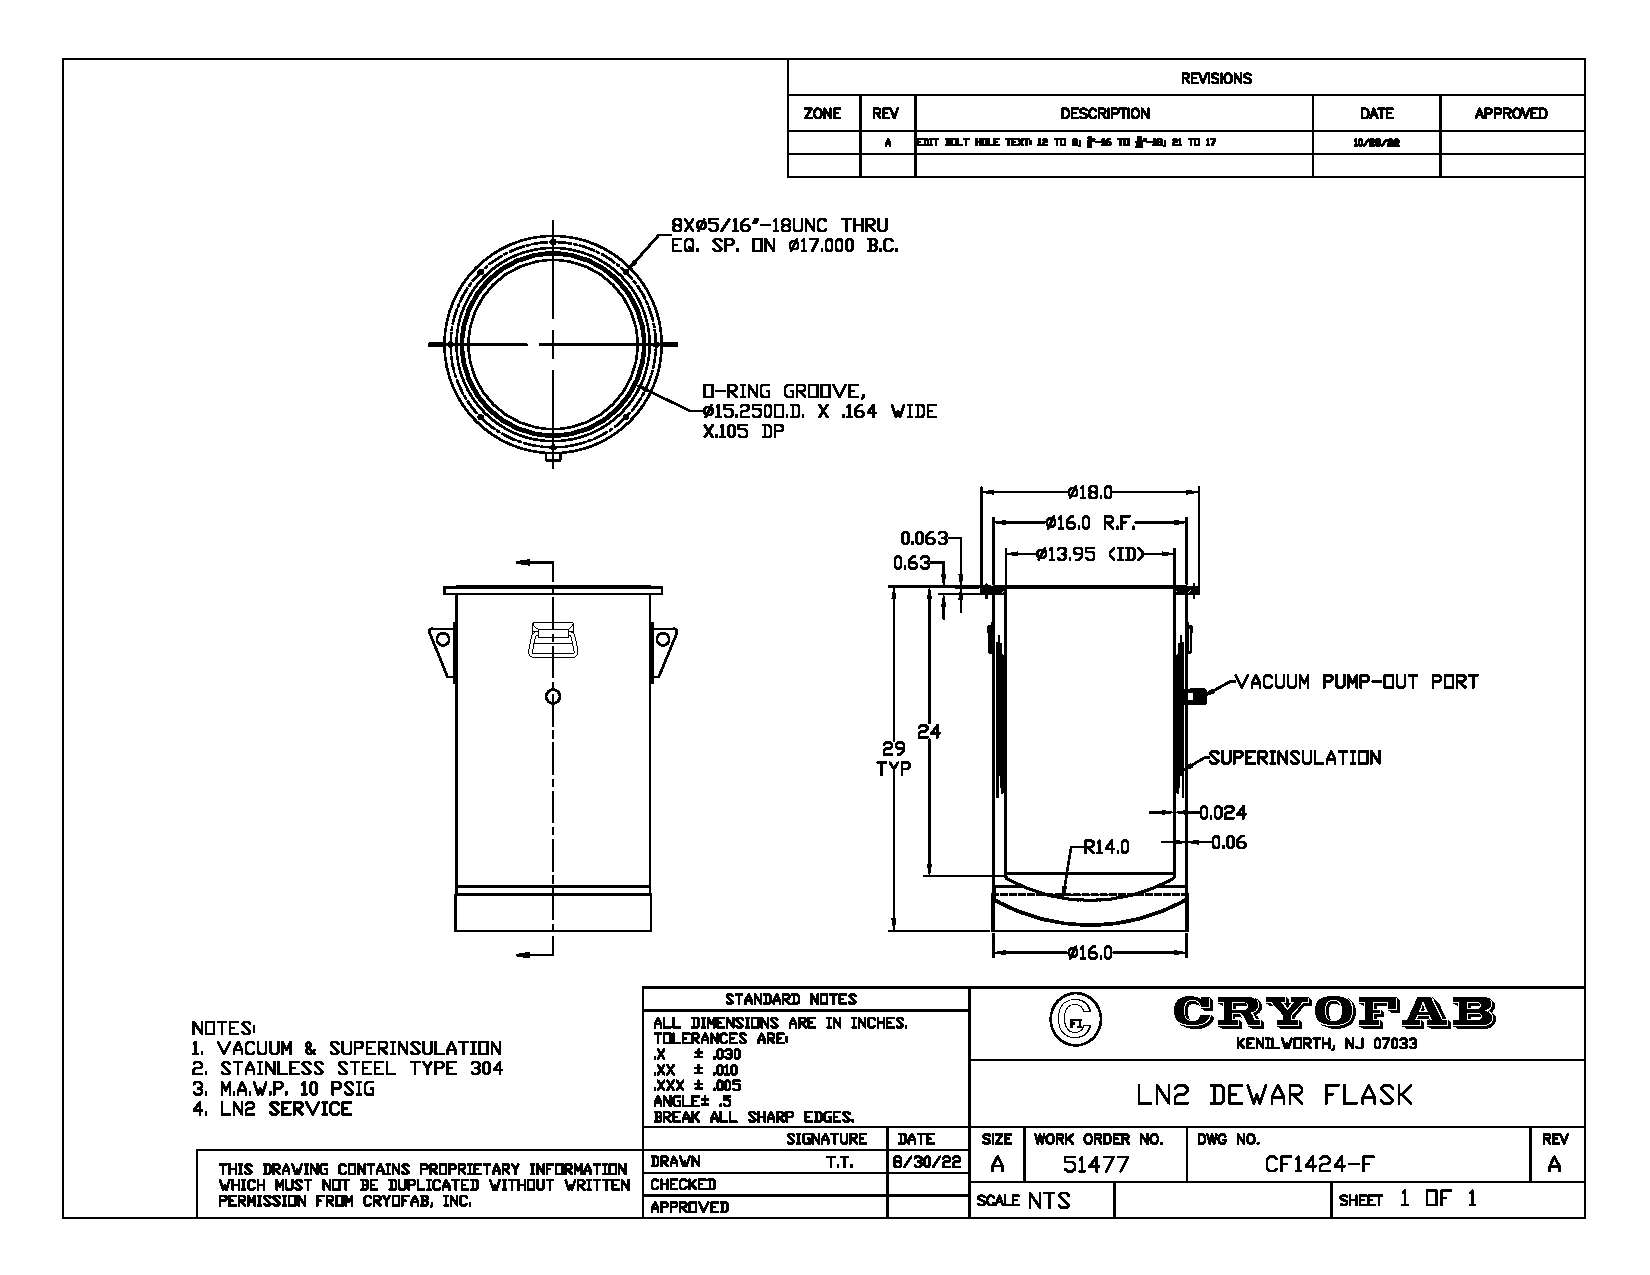
\includegraphics[width=\textwidth]{fig/DewarDrawing.pdf}
    \caption{Cryofab drawing of the CF 1424-F dewar.}
    \label{fig:dewar}
\end{figure}
% ----------------------------------------------------------


\clearpage
\section{Drawing of the Top Plate}
\label{app:top_plate_drawing}

\begin{figure}[h]
    \centering
    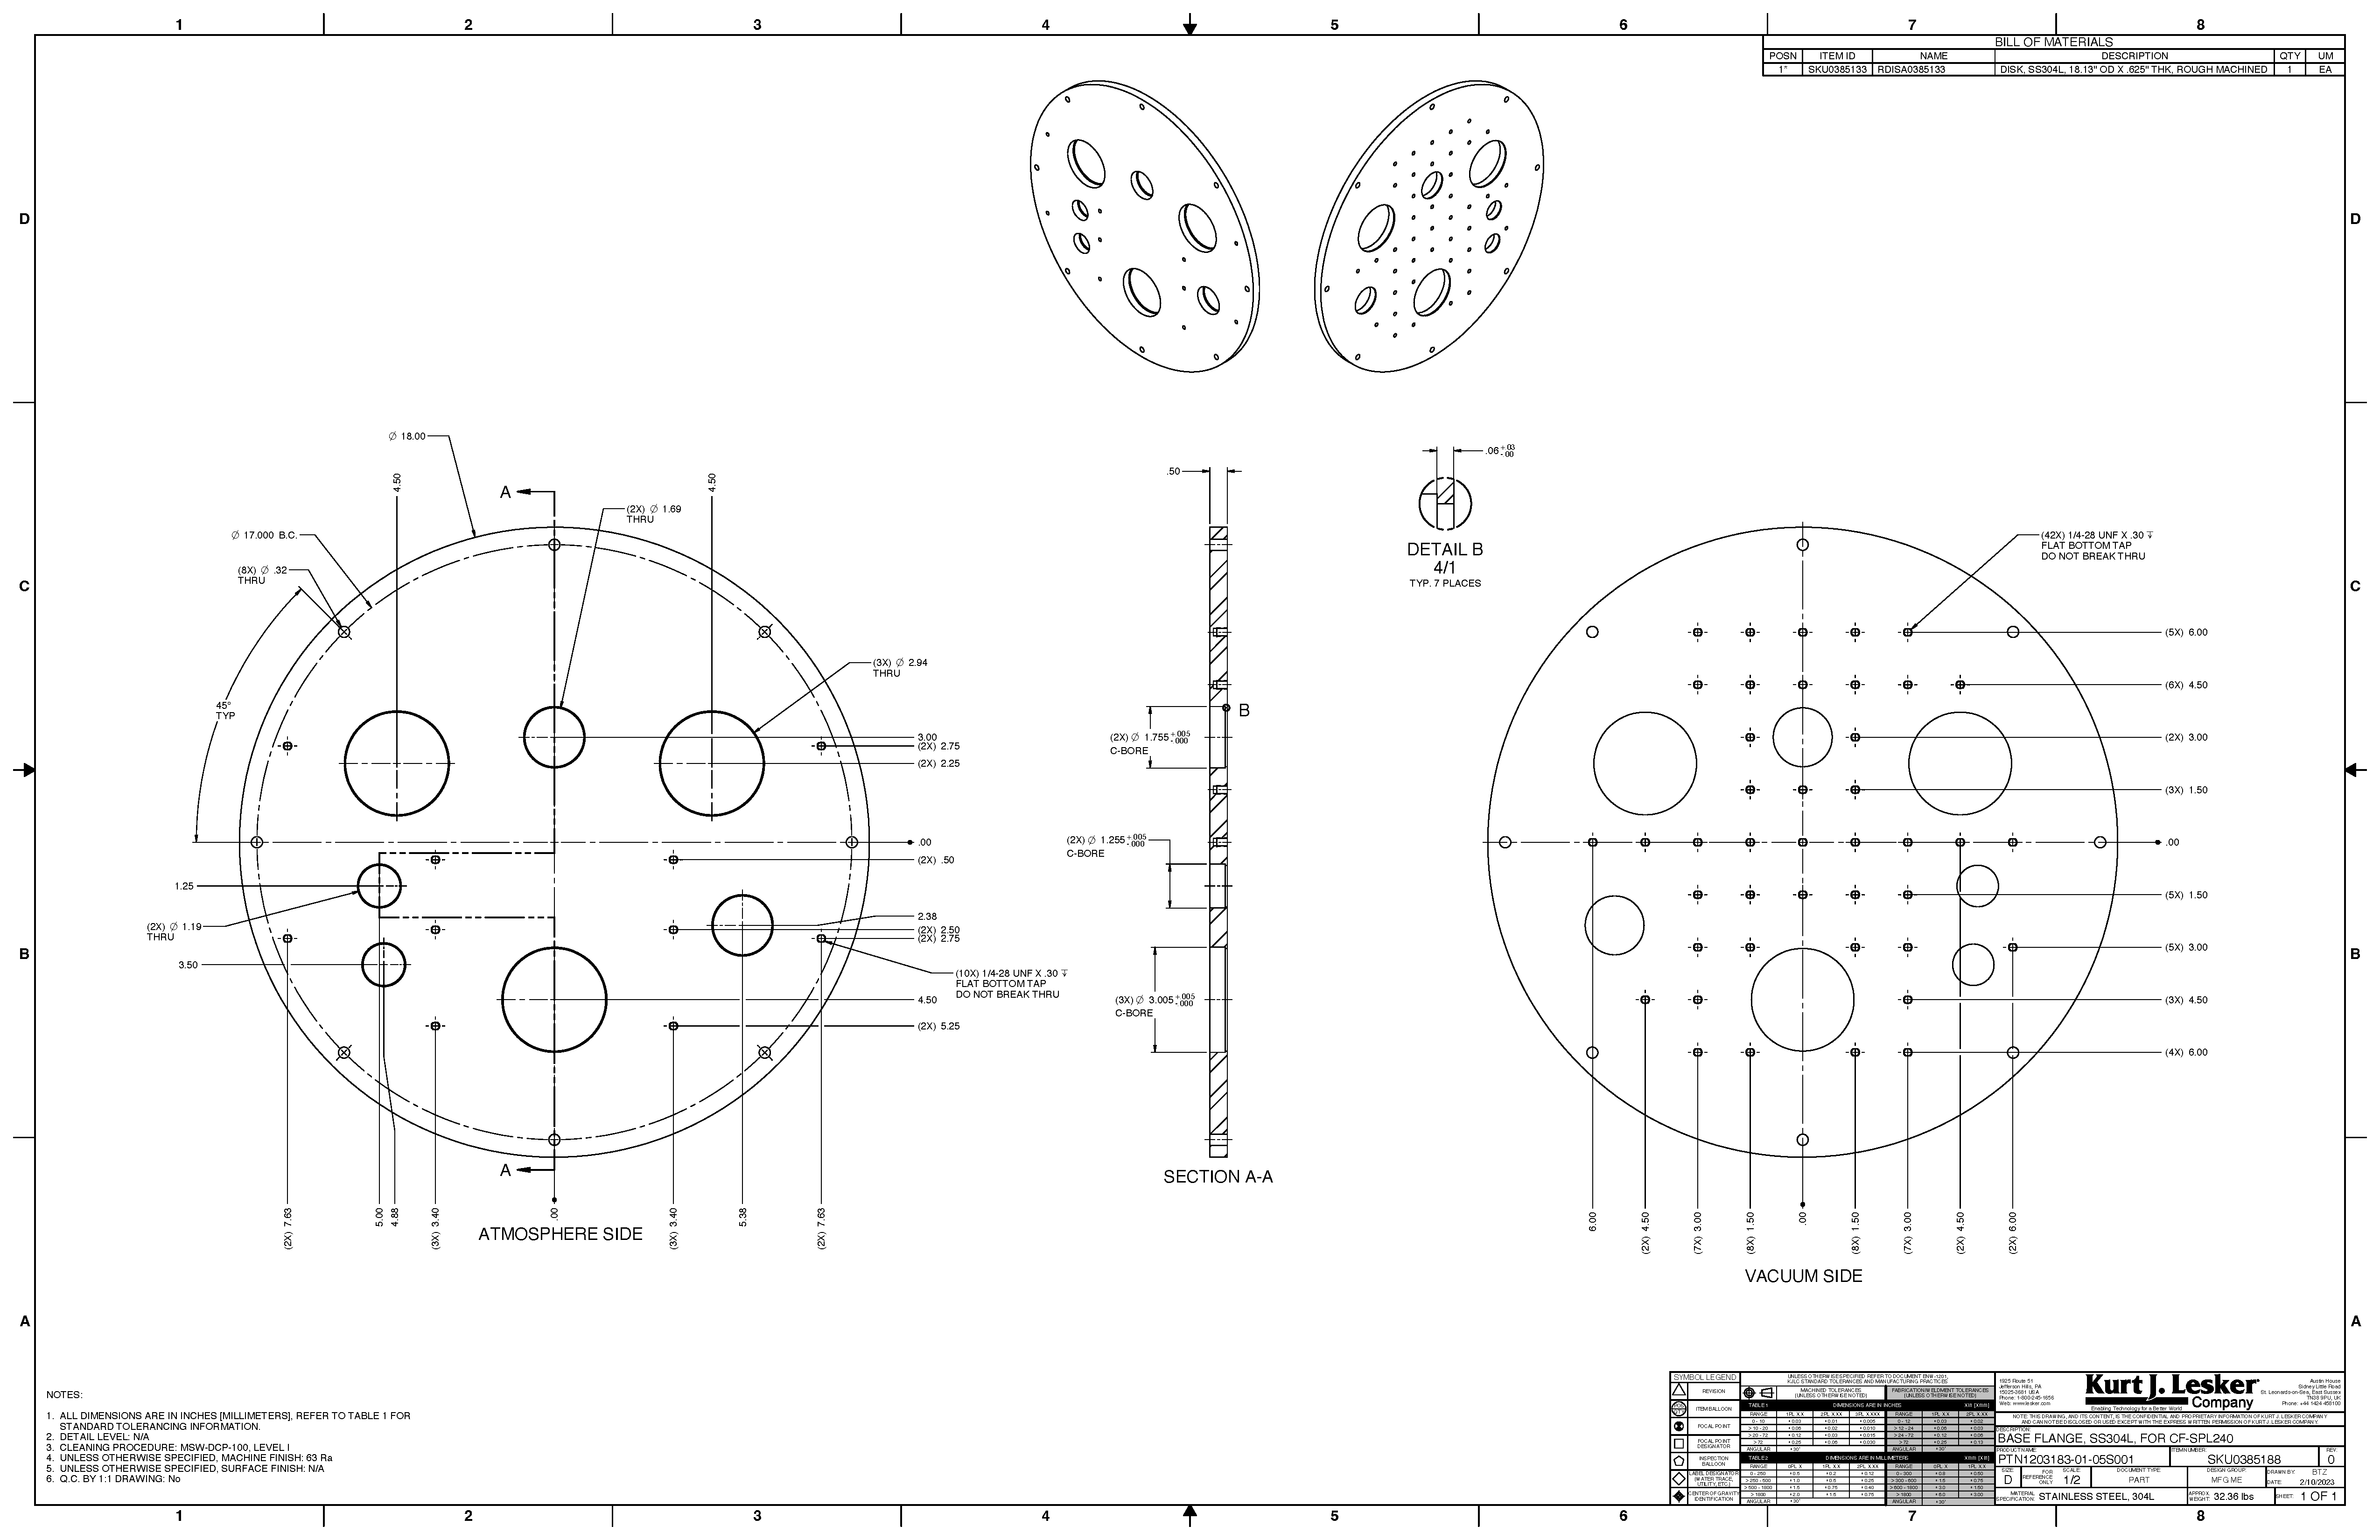
\includegraphics[width=\textwidth,angle=90]{fig/TopPlate.pdf}
    \caption{Drawing of the top plate.}
    \label{fig:top_plate}
\end{figure}

\clearpage
\section{Drawing of the Dewar}
\label{app:dewar_drawing}

\begin{figure}[h]
    \centering
    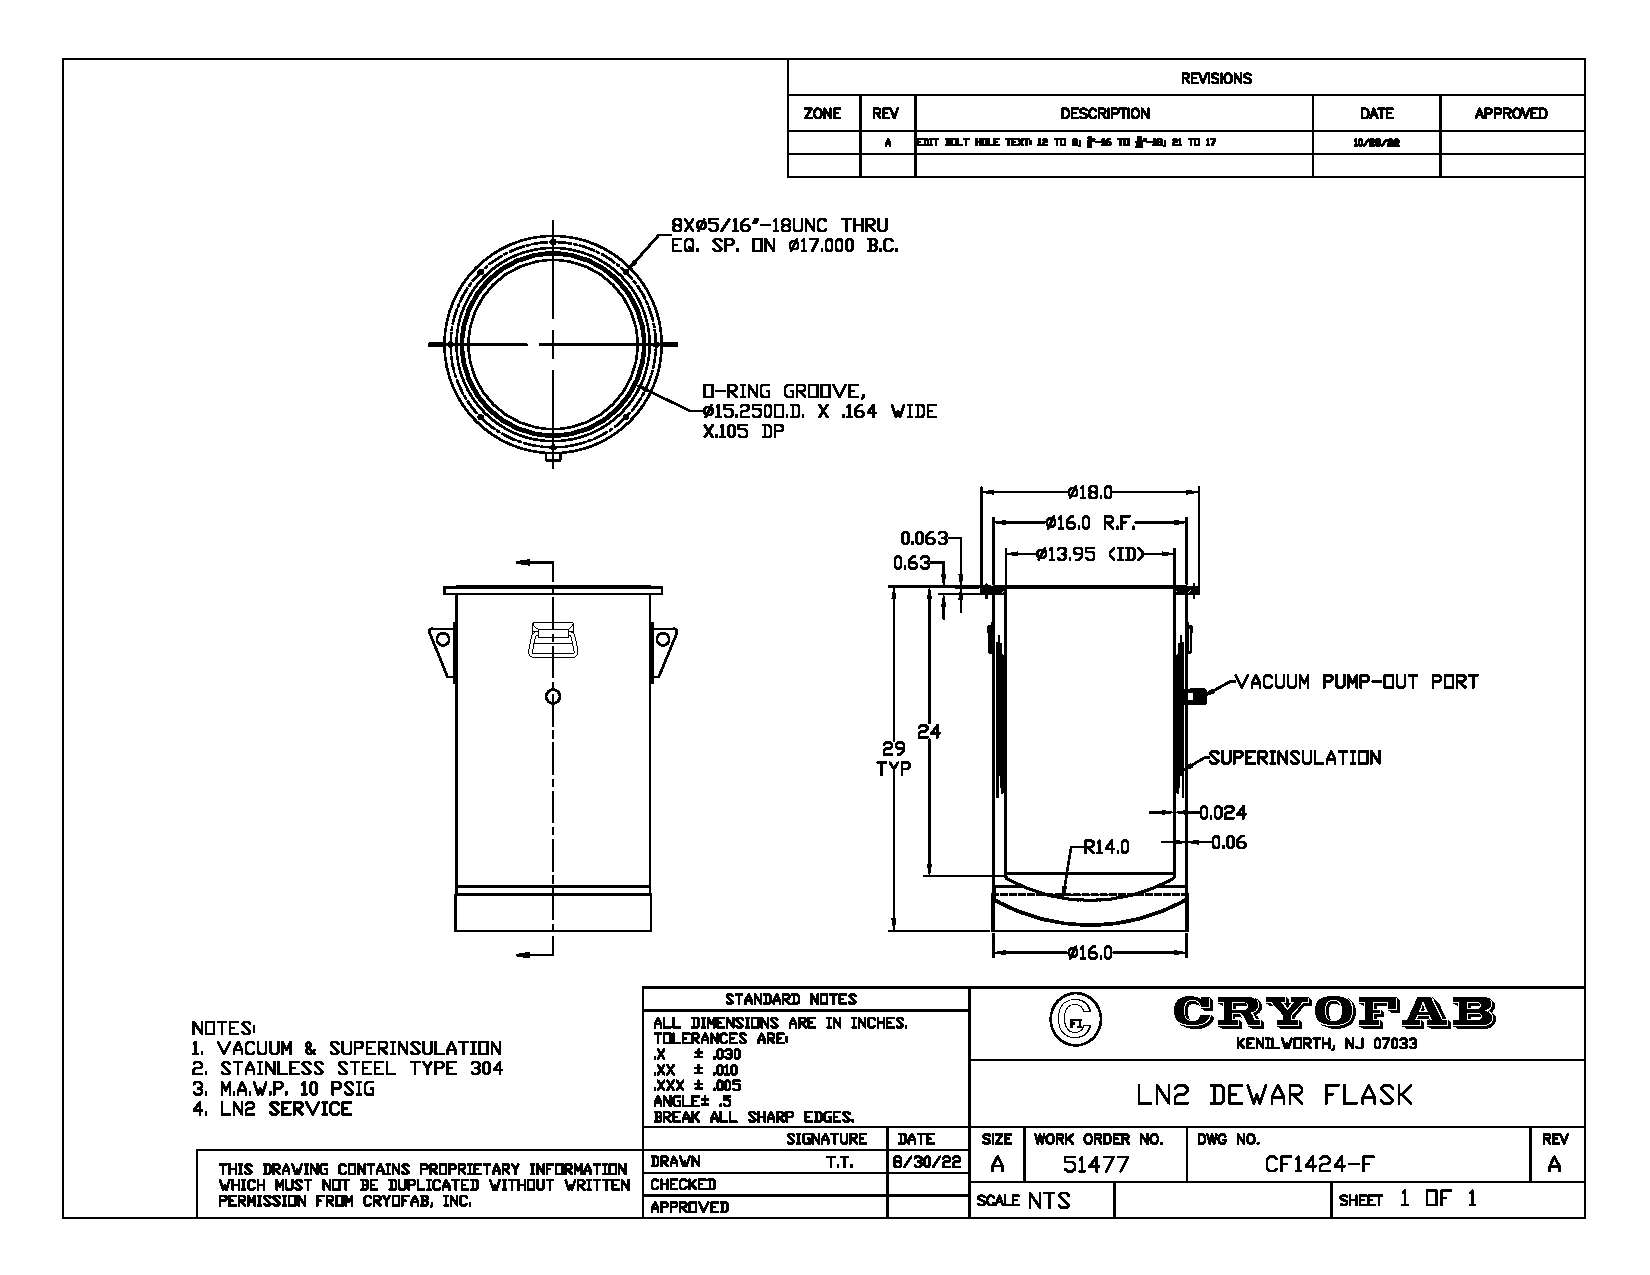
\includegraphics[width=\textwidth,angle=90]{fig/DewarDrawing.pdf}
    \caption{Cryofab drawing of the CF 1424-F dewar.}
    \label{fig:dewar}
\end{figure}

\clearpage
\section{Ring Flange Stress}
\label{app:ring_flange}

% SLArpaas has flat face flanges with metal-to-metal contact outside the bolt
% circle, and Figure~Y-5.1.3 in non-Mandatory Appendix~Y, Class~3 Flange Assembly
% applies.

The SLArpaas dewar and flange is made of stainless steel 304,
and the parameters are listed in Table~\ref{table:ring_flange}.
The calculations in this appendix can be found at
\url{https://github.com/yuntsebaryon/SLArpaasPressureAna/blob/main/notebook/RingFlangeStress.ipynb}.\\

%-------------------------------------------------------------------
\begin{table}[h]
\begin{center}
\tabcolsep=10pt
\begin{tabular}{r|c|l|l}
\hline
\hline
Variable & & Value & Unit \\
\hline
Outside diameter of flange & $A$ & 18 & in \\
Inside diameter of flange & $B$ & 14 & in \\
Bolt‐circle diameter & $C$ & 17 & in \\
Outside diameter of gasket contact face & $G$ & 15.086 & in \\
Flange thickness & $t$ & 0.63 & in \\
Number of bolts & $n$ & 8 & n/a \\
Internal design pressure & $P$ & 15 & psig \\
Nominal bolt diameter & $a$ & 0.313 & in \\
\hline
\hline
\end{tabular}
\caption{Flange parameters of the dewar based on the Cryofab drawing
and analysis.  Note that the flange thickness refers to the flange
of the dewar.  The nominal bolt diameter, $a$, is taken from 5/16"-18 bolts.}
\label{table:ring_flange}
\end{center}
\end{table}
%-------------------------------------------------------------------


% ----------------------------------------------------------------------
\subsection{Bolt Load}
\label{app:bolt_load}

SLArpaas has an O-ring, one of the self-energizing types (Table~2.5-1),
and therefore Mandatory Appendix~2 is referred herein.
The minimum required bolt load for the operating conditions,
$W_{m1}$, can be obtained following Eq.~2-5(c)(3)(-a) with $H_p = 0$,

\begin{equation}
    W_{m1} = H + H_p = H = 0.785G^2 P.
\end{equation}

$W_{m1}$ is 2282.2~pound.\\

The minimum required bolt load for gasket seating, $W_{m2}$, according to
2-5(c)(3)(-b), is 0.

% ----------------------------------------------------------------------
\subsection{Bolt Spacing}
\label{app:bolt_spacing}

According to 2-5(d), the maximum bolt space, $B_{s,max}$, can be obtained
by Eq.~2.5(d)(3)

\begin{equation}
    B_{s,max} = 2a + \frac{6t}{m+0.5}.
\end{equation}

The cord length of the bolt spacing on SLArpaas can be calculated with
\begin{equation}
    B_s = \frac{C}{2}\frac{\sin(2\pi/n)}{\sin((\pi-(2\pi/n))/2)}.
\end{equation}

The maximum bolt spacing $B_{s,max}$ therefore should be 8.186~in,
while SLArpaas has the bolt spacing 6.5~in.
The requirement is satisfied.

% ----------------------------------------------------------------------
\subsection{Bolt Area}
\label{app:bolt_area}

The specified minimum tensile strength at room temperature, $S_T$,
is 70000~psi in the Cryofab analysis.
The bolts on McMaster are mostly made of SAE J429, and the Grade 2
(low or medium carbon steel) with 1/4" - 3/4" size has the minimum 
tensile strength 74000~psi.
Therefore $S_T = 70000$~psi is a reasonable number.\\

The allowable bolt stress at design temperature (see UG-23), $S_b$,
is defined as $S_b = S_T/4$ in the Cryofab analysis.
This can be found in Table 6-100(a), 6-100(b), 6-100(c) in Section~II 
Part~D of the ASME code.\\

The total cross‐sectional area of bolts at root of thread or section 
of least diameter under stress,
required for the operating conditions, $A_{m1} = W_{m1}/S_b$.\\

The minimum required bolt area, $A_{m1} = 0.153~\text{in}^2$,
while the area of each bolt, $A_b$, is 0.045~in$^2$, according to
the Cryofab analysis.
Note that the area of a 5/16"-18 bolt is 0.077~in$^2$.
The total bolt area at SLArpaas is $A_bn = 0.045\times 8 = 0.36~\text{in}^2$,
satisfying the requirement ($>0.153~\text{in}^2$).

% ----------------------------------------------------------------------
\subsection{Flange Design Bolt Load}
\label{app:flange_bolt_load}

According to Mandatory Appendix 2-5(e) in the ASME code,
the flange design bolt load, $W$, can be obtained by

\begin{equation}
    W = W_{m1}
\end{equation}

for operating conditions, while

\begin{equation}
    W = \frac{(A_m+A_b)S_a}{2}
\label{eq:flange_bolt_load_gasket_seating}
\end{equation}

for gasket seating.
$S_a$ is allowable bolt stress at atmospheric temperature (UG-23).
Also 2-5(e) explains,

\begin{displayquote}
    Sa used in eq. (5) (Eq.~\ref{eq:flange_bolt_load_gasket_seating} herein) 
    shall be not less than that tabulated in the stress tables (see UG-23). 
    In addition to the minimum requirements for safety, eq. (5) provides 
    a margin against abuse of the flange from overbolting. 
    Since the margin against such abuse is needed primarily for the initial, 
    bolting‐up operation which is done at atmospheric temperature and before 
    application of internal pressure, the flange design is required to satisfy 
    this loading only under such conditions.
\end{displayquote}

In this specific case, $S_a = S_b$, $A_m = A_{m1}$.

The flange design bolt load is 4489.9~pound.

% ----------------------------------------------------------------------
\subsection{Flange Moment}
\label{app:flange_moment}

For the operating conditions, the total flange moment is described
in Appendix~2-6 in the ASME code,

\begin{equation}
    M_{op} = M_D+M_T+M_G,
\end{equation}

where $M_{op}$ is denoted as $M_o$ in the ASME code,
$M_D = H_Dh_D$, $M_T = H_Th_T$ and $M_G = H_Gh_G$.

All these variables can be found in Appendix~2-3 in the ASME code,
and are listed below.\\

$H_D$ = hydrostatic end force on area inside of flange \\
= $0.785B^2P$

$h_D$ = radial distance from the bolt circle, to the circle on which 
$H_D$ acts, as prescribed in Table 2-6 \\
= $(C-B)/2$

$H_T$ = difference between total hydrostatic end force and the hydrostatic 
end force on area inside of flange \\
= $H - H_D$

$h_T$ = radial distance from the bolt circle to the circle on which 
$H_T$ acts as prescribed in Table 2-6 \\ 
= $C/2 - (B/2+G/2)/2$

$H_G$ = gasket load for the operating condition \\
= $W_{m1} - H$

$h_G$ = radial distance from gasket load reaction to the bolt circle \\
= $(C-G)/2$ \\

Therefore, the total flange moment for the operating conditions
$M_{op} = 3918.78$~pound$\times$in.\\

For gasket seating, the total flange moment is calculated based on
Eq.~2-6(6) in the ASME code,

\begin{equation}
    M_a = W\frac{C-G}{2},
\end{equation}

where $M_a$ is denoted as $M_o$ in the ASME code.
$M_a = 4296.85$~pound$\times$in.

In Appendix~2-6 of the ASME code, it is stated,

\begin{displayquote}
    When the bolt spacing exceeds $2a + t$, multiply $M_O$ by the bolt spacing 
    correction factor $B_{SC}$ for calculating flange stress, where \\

    $B_{SC} = \sqrt{\frac{B_S}{2a+t}}$
\end{displayquote}

$B_{SC} = 2.28$ for the SLArpaas dewar.

% ----------------------------------------------------------------------
\subsection{Tangential Stress in Flange}
\label{app:tangential_stress}

The tangential stress, $S_T$, is defined in Appendix~2-7(b)(11) of the
ASME code,

\begin{equation}
    S_T = \frac{YM_o}{t^2B}.
\end{equation}


We calculate the operating conditions ($M_{op}$) with the bolt spacing 
factor, $B_{SC}$ applied,

\begin{equation}
    S_T = \frac{YM_{op}B_{SC}}{t^2B}.
\end{equation}

In addition, $Y$ is defined in Appendix~2-3 and Figure~2-7.1,

\begin{equation}
    Y = \frac{1}{K-1}[0.66845+5.7169\frac{K^2\log_{10}K}{K^2-1}],
\end{equation}

where $K = A/B$ is the ratio of outside diameter of flange to 
inside diameter of flange.

The tangential stress of the SLArpaas dewar flange is 12627.88~psi.
As the maximum allowable stress value in tension from applicable table
of stress values referenced by UG-23 (Table~ULT-23)
is 20~kpi = 20000~psi at temperature of 0, 100, 150$^{\circ}$F,
the tangential stress of the SLArpaas flange fulfils the requirement.


\clearpage
\section{Top Plate Design Pressure Calculations}
\label{app:top_plate}

The top plate of SLArpaas is made of stainless steel 304, and has
a thickness of 0.5~in, as shown in Fig.~\ref{fig:top_plate}.
All the calculations in this appendix can be found
at \url{https://github.com/yuntsebaryon/SLArpaasPressureAna/blob/main/notebook/TopFlangeStress.ipynb}.

\subsection{Minimum Required Top Plate Thickness}
\label{app:blind_flange}

The minimum required thickness for the top plate is calcuated assuming
a blind plate.  Eq. UG-34(c)(2)(1) below is used.

\begin{equation}
    t= d\sqrt{CP/SE}
\end{equation}

%-------------------------------------------------------------------
\begin{table}[h]
\begin{center}
\tabcolsep=10pt
\begin{tabular}{r|l|l|l}
\hline
\hline
Variable & Value & Unit & Reference \\
\hline
Diameter $d$ & 18 & in & design drawing \\
C & 0.25 & n/a & sketch (p) of Fig. UG-34 \\
P & 12.5 & psig & 10\% beyond the Cryofab spec. \\
S & 20000 & psi & Table ULT-23 at 0, 100, 150$^{\circ}$F \\
E & 1 & n/a & Table UW-12 \\
\hline
Minumum Required Thickness $t$ & 0.225 & in & UG-34 (c)(2)(1) \\
\hline
SLArpaas Top Plate Thickness & 0.5 & in & design drawing \\
\hline
\hline
\end{tabular}
\caption{Blind flange parameters to determine the minimum required thickness.}
\label{table:blind_flange}
\end{center}
\end{table}
%-------------------------------------------------------------------


The SLArpaas top plate has a thickness of 0.5~in, greater than the minimum
required thickness, 0.27~in.
In other words, with the thickness of 0.5~in, the blind SLArpaas top plate
can withstand the pressure of 51.44~psi.

% ----------------------------------------------------------------------
\subsection{Openings on the Top Plate}
\label{app:openings}

% ----------------------------------------------------------------------
\subsubsection{Welded Connections}
\label{app:welded}

The required minimum thickness of SLArpaas is 0.225~in, and therefore
UG-36(c)(3)(-a) applies,

\begin{displayquote}
    3 1/2 in. (89 mm) diameter -- in vessel shells or heads with a 
    required minimum thickness of 3/8~in. (10~mm) or less;
\end{displayquote}

The largest openings have the diameter of 3~in, 
and therefore no reinforcement is required for welded connections.

% ----------------------------------------------------------------------
\subsubsection{Reinforcement Required for Openings}
\label{app:opening_reinforcement}

The reinforcement requirements are based on UG-36(c)(3)(-c):

\begin{displayquote}
    no two isolated unreinforced openings, in accordance with (-a) 
    or (-b) above, shall have their centers closer to each other than 
    the sum of their diameters;
\end{displayquote}

Table~\ref{table:opening_dist} lists the distances of the openings on SLArpaas.

%-------------------------------------------------------------------
\begin{table}[h]
\begin{center}
\tabcolsep=10pt
\begin{tabular}{m{2cm}|m{2cm}|l|m{2cm}|m{2.5cm}}
\hline
\hline
Diameter of Opening 1 (in) & 
Diameter of Opening 2 (in) & Distance (in) & 
Required Distance (in) & 
Reinforcement Required? \\
\hline
3 & 3 & 8.113, 8.113, 9 & 6 & No \\
1.7 & 1.7 & 7.601 & 3.4 & No \\
1.2 & 1.2 & 2.253 & 2.4 & Yes (1) UG-39(b)(2) \\
3 & 1.2 & 3.536, 4.977 & 4.2 & Yes (2) UG-39(b)(2) \\
3 & 1.7 & 4.562 & 4.7 & Yes (3) UG-39 (b)(2) \\
3 & 1.7 & 4.707, 5.78 & 4.7 & No \\
\hline
\hline
\end{tabular}
\caption{Distances between the openings on the top plate of
SLArpaas, and the reinforcement requirements.}
\label{table:opening_dist}
\end{center}
\end{table}
%-------------------------------------------------------------------

The total cross-section area of the reinforcement is given by 
Eq.~UG-39(b)(1),

\begin{equation}
    A = 0.5dt + tt_n(1-f_{r1}),
\end{equation}

where $f_{r1}$ is defined in UG-37. 
As this case corresponds to sketch (o) in Figure~UG-40,
$f_{r1} = 1$.
Therefore the total cross-section area of the reinforcement becomes,

\begin{equation}
    A = 0.5dt,
\end{equation}
where $t$ is the minimum required thickness, 0.225~in,
and $d$ is finished diameter of circular opening or finished dimension 
(chord length at mid-surface of thickness excluding excess thickness 
available for reinforcement) of nonradial opening in the plane under 
consideration, in. (mm) (UG-37).

The reinforcement requirements can be found in UG-39(b)(2),

\begin{displayquote}
    Multiple openings none of which have diameters exceeding one‐half 
    the head diameter and no pair having an average diameter greater 
    than one‐quarter the head diameter may be reinforced individually 
    as required by (1) above when the spacing between any pair of 
    adjacent openings is equal to or greater than twice the average 
    diameter of the pair.\\

    When spacing between adjacent openings is less than twice but equal 
    to or more than 1 1/4 the average diameter of the pair, the required 
    reinforcement for each opening in the pair, as determined by (1) 
    above, shall be summed together and then distributed such that 50\% 
    of the sum is located between the two openings. 
    Spacings of less than 1 1/4 the average diameter of adjacent openings 
    shall be treated by rules of U-2(g).
\end{displayquote}

The existing reinforcement is greater than the shortest distance 
between the two openings times the extra top plate thickness
with respect to the minimum required thickness $t$,

\begin{equation}
    R = (s - \davg)\times(\tslarpaas-t).
\end{equation}

$s$ is the distance between the centers of the two openings,
$\davg$ is the average diameter of the two openings,
and $\tslarpaas$ is the actual thickness of the top plate.
Reinforcement is fulfiled if $R$ is greater than $0.5A$,
where $A = 0.5\davg t$ when the two openings have different 
diameters.
Table~\ref{table:opening_reinforcement} shows the parameters
and the calculation results of the openings requiring 
reinforcement.

%-------------------------------------------------------------------
\begin{table}[h]
\begin{center}
\tabcolsep=10pt
\begin{tabular}{l|m{2cm}|m{2cm}|m{1.4cm}|l|l|m{2.2cm}}
\hline
\hline
No. & Diameter of Opening 1 (in) & 
Diameter of Opening 2 (in) & 
Distance $s$ (in) &
$A$ (in$^2$) & $R$ (in$^2$) & Reinforcement Fulfiled? \\
\hline
(1) & 1.2 & 1.2 & 2.253 & 0.135 & 0.289575 & Yes \\
(2) & 3 & 1.2 & 3.536 & 0.23625 & 0.3949   & Yes \\
(3) & 3 & 1.7 & 4.562 & 0.264375 & 0.6083  & Yes \\
\hline
\hline
\end{tabular}
\caption{Calculation of required reinforcements.  The numbering 
corresponds to Table~\ref{table:opening_dist}. }
\label{table:opening_reinforcement}
\end{center}
\end{table}
%-------------------------------------------------------------------

In summary, the reinforcement requirements are satisfied for
all the openings.


\end{appendices}

\end{document}